% !TeX spellcheck = en_US
\documentclass[10pt]{../imeko_acta}
\usepackage{siunitx}
\sisetup{per-mode = symbol}

\author[1]{Rocío Alejandra Guerrón}
\author[2]{Francesco D'Amore}
\author[2]{Mariantonia Bencardino}
\author[1,3]{Francesco Lamonaca}
\author[4]{Antonio Colaprico}
\author[1]{Marco Lanuzza}
\author[1]{Ramiro Taco}
\author[1]{Domenico Luca Carnì}
\affiliation[1]{Department of Computer, Modeling, Electronics and Systems Engineering - University of Calabria, Rende, Italy}
\affiliation[2]{National Research Council of Italy, Istituto di Calcolo e Reti ad alte prestazioni (CNR-ICAR), Rende, Italy}
\affiliation[3]{National Research Council of Italy, Institute of Nanotechnology (CNR-NANOTEC), Rende, Italy}
\affiliation[4]{Department of Public Health Sciences, University of Miami Miller School of Medicine, Miami, FL, 33136, USA}


\CorrespondingAuthorNumber{1}
\CorrespondingAuthorEmail{alejandra.guerron@dimes.unical.it}

% Keywords - if you don't want any simply remove all the text between the curly brackets
\Keywords{Air quality;  sensor node architecture;  distributed measurement system; low-cost sensor; pollutants;  IoT} 

%Leave blank for no funding
\Funding{This research was funded by PNRR project: Tech4You "Spoke 2 - Technologies to reduce 372
	energy consumption and save biodiversity" and "Spoke 4 - Technologies for resilient and accessible 373
	cultural and natural heritage".}
%Leave blank for no funding, like this
%\Funding{}

%----------------------------------------------------------------
% Completed by Editors - You can fill in but Editor will finalize
%----------------------------------------------------------------
\Editor{Francesco Lamonaca}
\EditorAffiliation{University of Calabria, Italy}
\Received{January 1, 2021}
\FinalForm{January 31, 2021}
\Published{March 6, 2021}
\VolumeNumber{12}
\VolumeMonth{December}
\VolumeYear{2023}
\IssueNumber{4}
\ArticleNumber{26}
\SubmissionNumber{1676}
%\PageNumbers{1 - 10}
%\Authors{Rocío Alejandra Guerrón; Francesco D'Amore; Mariantonia Bencardino; Francesco Lamonaca; Antonio Colaprico; Marco Lanuzza; Ramiro Taco; Domenico Luca Carnì}
%\Identifier{IMEKO-ACTA-12 (2023)-04-26}
%\Subject{Acta IMEKO 12 (2023) 4, 1-10}

%----------------------------------------------------------------------------------------
% Completed by Authors - Everything below here
%
\PaperTitle{IoT sensor nodes for air pollution monitoring: a review} % Article title

%----------------------------------------------------------------------------------------
%	ABSTRACT - Fill in with abstract - length less than 200 words. 
%----------------------------------------------------------------------------------------

\Abstract{Air quality is an important environmental concern, as it is strictly related to human health risks and adverse effects on it. Monitoring air pollutants and different ancillary parameters is a feasible and crucial approach to address this challenge. This task typically involves high expenses in case measurements are carried out by using conventional measurement instruments and human operators. However, utilizing measurement systems with low-cost sensors can reduce the overall implementation effort. The aim of this paper is to describe the sensor node architecture applicable to a general monitoring system and based on this structure, review different current low-cost measurement system proposals for outdoor air quality monitoring.
}

%----------------------------------------------------------------------------------------

\begin{document}
\maketitle % Print the title and abstract box


%-----------------------------------------------------------------------------------------

%----------------------------------------------------------------------------------------
%	ARTICLE CONTENTS
%----------------------------------------------------------------------------------------


\section{Introduction}

Air quality holds keen relevance for humans as it profoundly affects our health, exposing us to various risks and adverse effects. In fact, poor air quality can result in detrimental health consequences, particularly impacting the human respiratory system and heart heal-th, even potentially leading to fatalities~\cite{ROVIRA2020135538}. Recently, the World Health Organization (WHO) presented alarming statistics, stating that both ambient and household air pollution cause at least 6.7 million premature deaths per year. Furthermore, 99\% of the world's population in 2019 lived in places where the health-based air quality levels recommended by WHO guidelines were not met~\cite{who_key}. Unlike water, the air that people inhale is not provided through a controlled or centralized source that regulates its quality or ensures it meets minimum standards for human health~\cite{WHO}. 
 
The most common atmospheric pollutants that pose significant concerns for the air include nitrogen dioxide (NO$_{2}$), sulfur dioxide (SO$_{2}$), carbon monoxide (CO), ozone (O$_{3}$) as well as particulate matter categorized into two size fractions, named as PM$_{2.5}$ and PM$_{10}$, with aerodynamic diameter lower than 2.5 and 10~\unit{\micro \meter}, respectively~\cite{WHO}.

The primary sources of anthropogenic air pollution stem from the combustion of fossil fuels within the energy and industry sectors. Additionally, significant contributions arise from on-road transportation and international shipping. Other notable sources of air pollutants include residential heating, agriculture, and waste management sectors~\cite{essd-12-3413-2020}.

A viable strategy for mitigating air pollution involves two key aspects. Firstly, raising awareness about the impacts of air pollution is crucial. This helps individuals and communities to understand the consequences and motivates them to take action. Secondly, it is essential to identify the factors that contribute to air pollution. By recognizing the causes behind pollution, governments, private and public entities, and citizens can implement effective mitigation strategies~\cite{sofia}.

Unfortunately, gathering and processing information about air quality depends on economic, technological, and geographic factors. Air quality monitoring systems, with regulated environmental programs, need to comply with certain standard methods and technical protocols, depending on the country where they are going to be used. Constant calibration of sensor nodes and maintenance rules are needed to guarantee the accuracy of these systems, so they can provide reliable data of contaminants.
Therefore, it can be inferred that, in general, developed countries tend to allocate more public or private investments toward the collection, analysis, and subsequent action based on environmental data. In contrast, developing countries may face challenges in accessing sufficient or even non-existent environmental information~\cite{BALDASANO}.
In this scenario, the employment of low-cost sensors for measuring air pollutants and meteorological parameters emerges as a compelling and practical solution to bridge the economic gap. The use of low-cost sensors offers multiple advantages, such as the potential for increased monitoring locations, cost reduction, and even real-time data acquisition \cite{atmos10090506}. By leveraging these sensors, it becomes feasible to expand the monitoring network and gather valuable information to address air pollution challenges effectively.

Despite the wide range of low-cost sensors available in the market, there is a notable lack of information concerning their calibration, evaluation, and accuracy~\cite{LIU2020109438}. Additionally, their useful lifespan is still unclear. Many of these sensors exhibit low accuracy primarily because they are not designed to detect and measure specific gases, leading to cross-sensitivity issues~\cite{atmos10090506}. Due to the availability of a large number of commercial options and the limited data on their performance, it becomes crucial to analyze the key characteristics that define the outcomes of such sensors.

In conjunction with selecting suitable sensors, it is crucial to properly design the architecture of the wireless sensor node. The sensor node should have the capability to collect, process and transmit the acquired data to a central server, while also meeting power consumption requirements to fully leverage the potential of the Internet of Things (IoT) paradigm~\cite{suryavansh2021data, 5522465}. Consequently, an ideal sensor node is expected to comprise a multi-sensor electronic system that is wireless, cost-effective, and energy-efficient.

In order to provide an overview of the state of research and development of low-cost environmental monitoring systems, this paper will discuss the IoT sensor node's architecture and the state of the art of the recently developed systems. Therefore, the structure of this paper is the following: preliminary, the general architecture of the sensor node will be discussed; successively, state of art and analysis of systems presented in the last years will be summarized. Finally, discussions and conclusion remarks follow.

\section{Sensor Node Architecture}
A sensor node is an autonomous, small, portable, low-cost, and low-energy consumption device with limited resources~\cite{TENG2012251, STANKOVIC2013223}. Sensor nodes are capable of sensing physical changes, processing and transmitting the collected information~\cite{1197877, 9764728}. Considering the characteristics and capabilities of sensor nodes, it is possible to generate a smart environment suitable for a wide variety of industries such as livestock monitoring, surveillance,  military and national defense applications, smart homes, medical systems, transportation, meteorological, environmental monitoring systems and many others~\cite{1197877, 6859717, farha2010middleware, 5639549}.

Figure~\ref{sensor_node} illustrates a typical sensor node architecture, where the main components are: the sensing unit, the processor, the external memory, the transceiver, and the power supply unit. 

\begin{figure}[!tb]
	\centering
	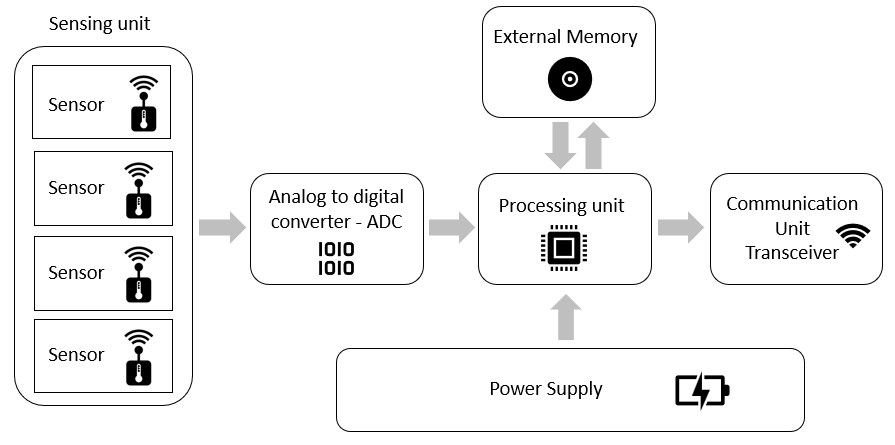
\includegraphics[width=\linewidth]{sensor_node_architectutre.png}
%	\vspace*{6pt}
	\caption{Sensor node architecture.}
	\label{sensor_node}
\end{figure}

The sensing unit comprises one or multiple sensors responsible for gathering data from the target environment for analysis~\cite{1197877, 6949922,9538816}.

Normally, this data needs to be digitized by an analog-to-digital converter (ADC). To process the collected data a processing unit is required such as a microprocessor, a microcontroller, a digital signal processor, or an application-specific integrated circuit depending on the needs, resources, and budget~\cite{6861346, 6949922}. External memory is necessary, either to store data related to the designed application and user data or for saving information required to program the processing unit~\cite{6949922}. A transceiver is indispensable for the communication of the sensor node towards other nearby sensor nodes. Finally, the power source unit is needed to provide power to the entire module.
Although batteries may be the most commercial and widely used option, they tend to run out quickly, requiring frequent replacement, which can occur after few days or years, it may be after a few days or years, depending on the number of sensors, processing, or communication unit handled by the sensor node~\cite{5339410}. For this reason, using energy from other sources, such as solar energy combined with an energy storage system, could be an alternative to incorporate in the power supply unit~\cite{5339410}.	

\section{Analysis of the architecture of the air quality systems}

To perform a comprehensive analysis of state-of-the-art of air quality monitoring systems, a thorough search was performed on publications related to the topic. In the research, the main articles database used are Scopus, IEEE explorer and  Google Scholar. The selection criteria of the article in the database were specified based on the topic of interest and objectives of this paper. The result of this search yielded a total of 27 selected works~\cite{JABBAR2022100540, liu2016low,wivou2016air,yang2015smart,gunawan2018design, purkayastha2021iot, kadir2021cloud, truong2021design, spandonidis2020compact,kumar2017air,sun2016development,de2020iot,PALOMEQUEMANGUT2022135948, s22020502, 8663367, chaudhari2017iot, zakaria2018wireless, deshmukh2016low, kaur2016air, pal2023remote, al2015monitoring, brienza2015low, phala2016air, kumar2020design, ahmed2017real, khedo2017low, fioccola2016polluino}, that met the following criteria:
\begin{itemize}
    \item Only publications from the last 8 years were considered.
    \item Given the purposes of this work, systems that address outdoor air quality monitoring are analyzed. It is important to mention that systems that can monitor both outdoors and indoors are also included, the only ones that are excluded are those intended for specifically indoor measurements.
    \item Only air quality monitoring systems developed by the authors of the research were considered. 
    \item Systems must monitor the concentration of at least one environmental pollutant.
    \item Only those contaminants that are monitored in at least two of the systems chosen for study are part of this analysis.
\end{itemize}

Considered works were published between 2015 and the first quarter of 2023. As shown in Figure~\ref{publications_year}, 2016 was the year in which the largest number of research papers were published. However,  in the following years, the percentage of publications with the desired characteristics decreased.

\begin{figure}[!tb]
	\centering
	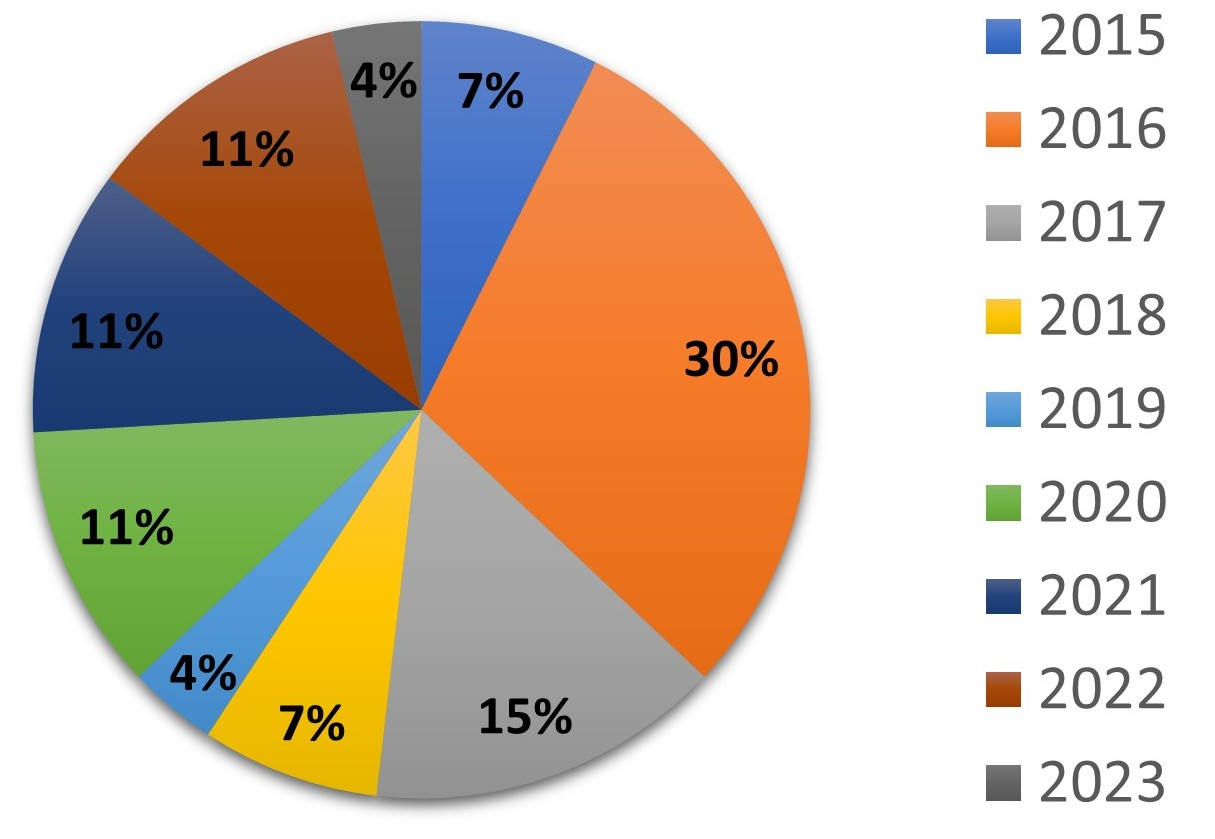
\includegraphics[width=0.7\linewidth]{number_papers_year.jpg}
%	\vspace*{6pt}
	\caption{Percentage of publications per year.
        \label{publications_year}}
\end{figure}

Among the systems, 21 were developed only for the outdoors, and the remaining 6 for both indoor and outdoor environments. Four different types of developed systems were found: fixed, portable, mobile, and wearable. Fixed systems are designed to be located in a single position, while portable ones are easy to move from one location to another. In both cases, the measurements are made with the equipment stationary and without movement. In a different way, wearable systems are very small and are developed to take measurements while the person is moving. Similarly, mobile systems are designed to measure environmental factors while a manned or unmanned vehicle is in movement, such as a car, bus, or drone. 
 As depicted in Figure~\ref{type_systems}, fixed systems are the most predominant types, whereas wearable systems are the least represented.

 \begin{figure}[!tb]
	\centering
	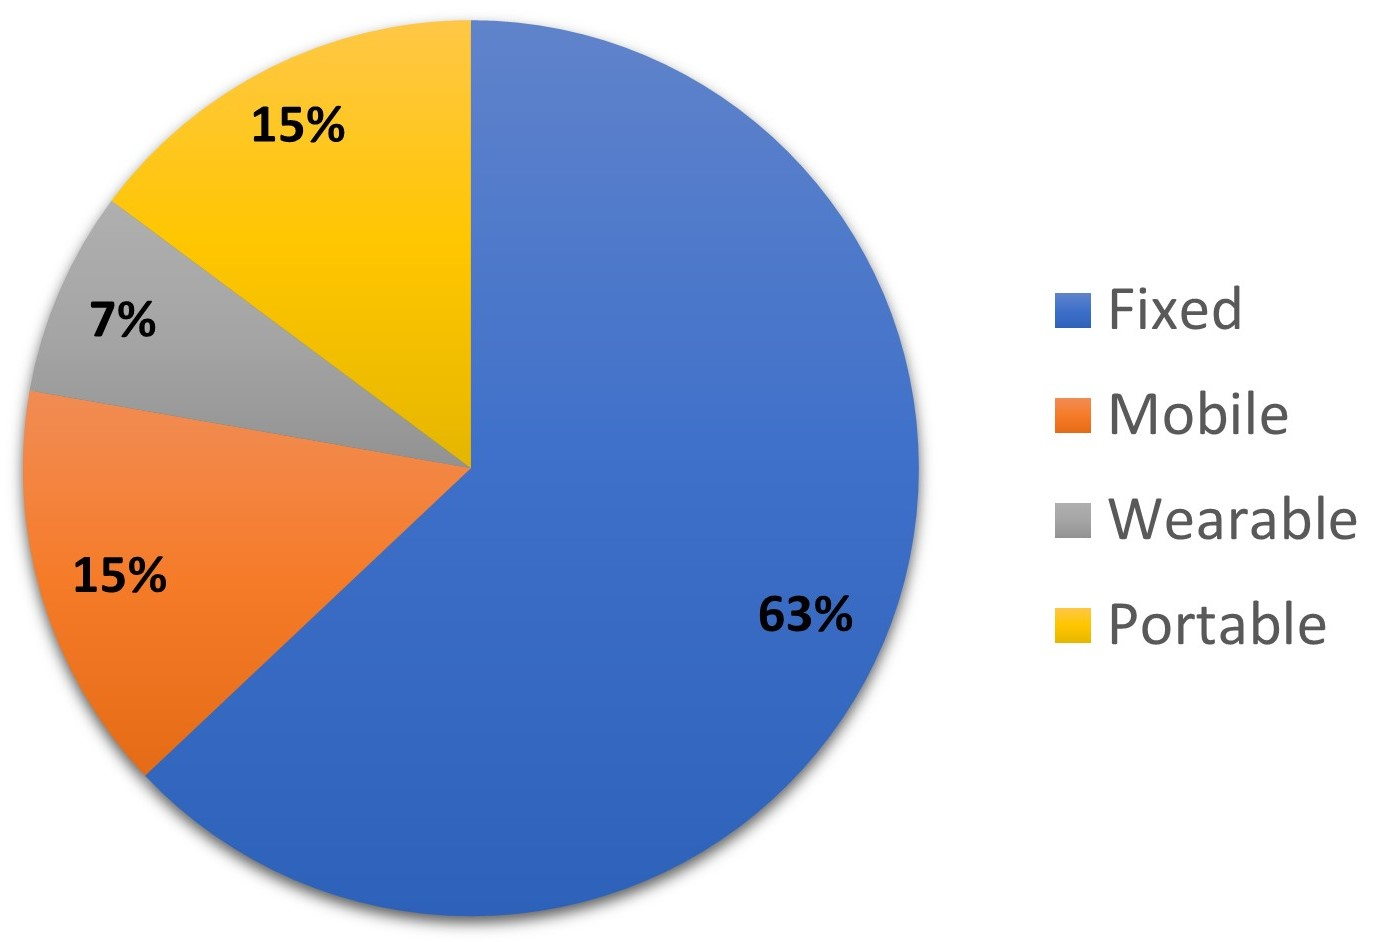
\includegraphics[width=0.7\linewidth]{type_of_system.jpg}
%	\vspace*{6pt}
	\caption{Types of systems.
        \label{type_systems}}
\end{figure}

By the analysis of the articles, only in 7 publications, it was mentioned that validation with one or more calibrated and reference devices was carried out to verify the results obtained by the systems. The remaining works solely  presented the results of their sensors as valid.

\subsection{Sensing Unit Analysis}\label{SUA}

Different pollutants and environmental factors were in the scope of the analyzed systems. The currently prevalent monitoring systems utilize expensive and bulky infrared and UV fluorescence analyzers, which are not conducive to the creation of low-cost and mobile systems that are the objective of this analysis. For this reason, this research will exclusively focus on the proposed low-cost use in air monitoring system architecture. The sensing unit will consider temperature and humidity sensors, gas sensors, and particular matter sensors. 

The environmental temperature was considered in 18 of the systems. Table~\ref{tabTemp} shows a summary of the most commonly utilized sensors along with their operating range and accuracy. It should be noted that only one of the sensors in Table~\ref{tabTemp} supplies an analog output which must therefore be suitably excited and conditioned, and it is the AD-590. While all the other sensors feature a digital output, therefore they integrate the conditioning system inside them.

\begin{table}[!tb]
	\caption{Temperature sensors.}
	\label{tabTemp}
	\centering
\begin{tabularx}{\columnwidth}{lCCC}
	\toprule
	Sensor	& Occurrences	& Ope.Range (\unit{\degreeCelsius}) & Accuracy (\unit{\degreeCelsius})\\
	\midrule
		DHT11~\cite{dht11}      & 4     &   0, 50        & $\pm$2  \\
		DHT22~\cite{dht22}      & 4     &   -40.0, 80.0  & $\pm$0.5  \\
		LM35~\cite{lm35}        & 3     &   0.0, 100.0   & $\pm$0.5  \\
		BME280~\cite{BME280}    & 2     & -40.0, 85.0    & $\pm$0.5 \\
		BME680~\cite{BME680}    & 2     & -40, 85        & $\pm$1 \\
		AD-590~\cite{ad590}     & 1     & -65, 155       & $\pm$3  \\
		DS18B20~\cite{ds18b20}  & 1     & -55.0, 125.0   & $\pm$0.5 \\
		SHT25~\cite{sht25}      & 1     & -40.0, 125.0   & $\pm$0.2 \\
	\bottomrule
\end{tabularx}
\end{table}

A similar scenario can be observed for humidity, where 16 systems considered measuring this parameter. Table~\ref{tabHum} shows the humidity sensors that were used in the analyzed systems. Also in this case, most of the sensors shown in Table~\ref{tabHum} have a digital output, therefore already conditioned, except for the SY-HS220 and HIH-4030 sensors which provide an analog output.

\begin{table}[!tb]
	\caption{Humidity sensors.}
	\label{tabHum}
	\centering
\begin{tabularx}{\columnwidth}{lCCC}
	\toprule
	Sensor	& Occurrences	& Ope.Range (\unit{\percent}) & Accuracy (\unit{\percent})\\
	\midrule
	DHT11~\cite{dht11}      & 5 &  20, 90       & $\pm$5\\
	DHT22~\cite{dht22}      & 4 & 0, 100        & $\pm$2 \\
	BME280~\cite{BME280}    & 2 & 0, 100        & $\pm$3  \\
	BME680~\cite{BME680}    & 2 & 0, 100        & $\pm$3 \\
	SHT-25~\cite{sht25}     & 1 & 0.0,100.0     & $\pm$1.8  \\
	SY-HS220~\cite{SYHS220} & 1 & 30, 90        & $\pm$5 \\
	HIH-4030~\cite{HIH4030} & 1 & 0.0, 100.0    & $\pm$3.5 \\
	\bottomrule
\end{tabularx}
\end{table}

From the presented findings, the systems which took measurements of humidity also did for temperature, but not vice versa.  The most used sensors to measure both temperature and relative humidity were DHT11 and the DHT22. As mentioned in~\cite{9826978}, these two sensors are low-cost, digital, and show a difference based on the operating ranges and accuracy. DHT22 has a wider operating range and better accuracy than DHT11. Regarding to pressure, it was only measured in the 18.52\% of the systems, represented only by three devices from the same brand: BME180, BME280, and BME680, which were also used for temperature and humidity sensing.

Within the sensor unit, 10 different contaminant gases were considered in the selected systems. Figure~\ref{occurrences_pollutants} illustrates that CO, NO$_{2}$, CO$_{2}$, and O$_{3}$ were the most measured gases across the studied systems. Apart from SO$_2$, these listed contaminants correspond aptly with the most common pollutants ruled by air quality directives.

\begin{figure}
	\centering
	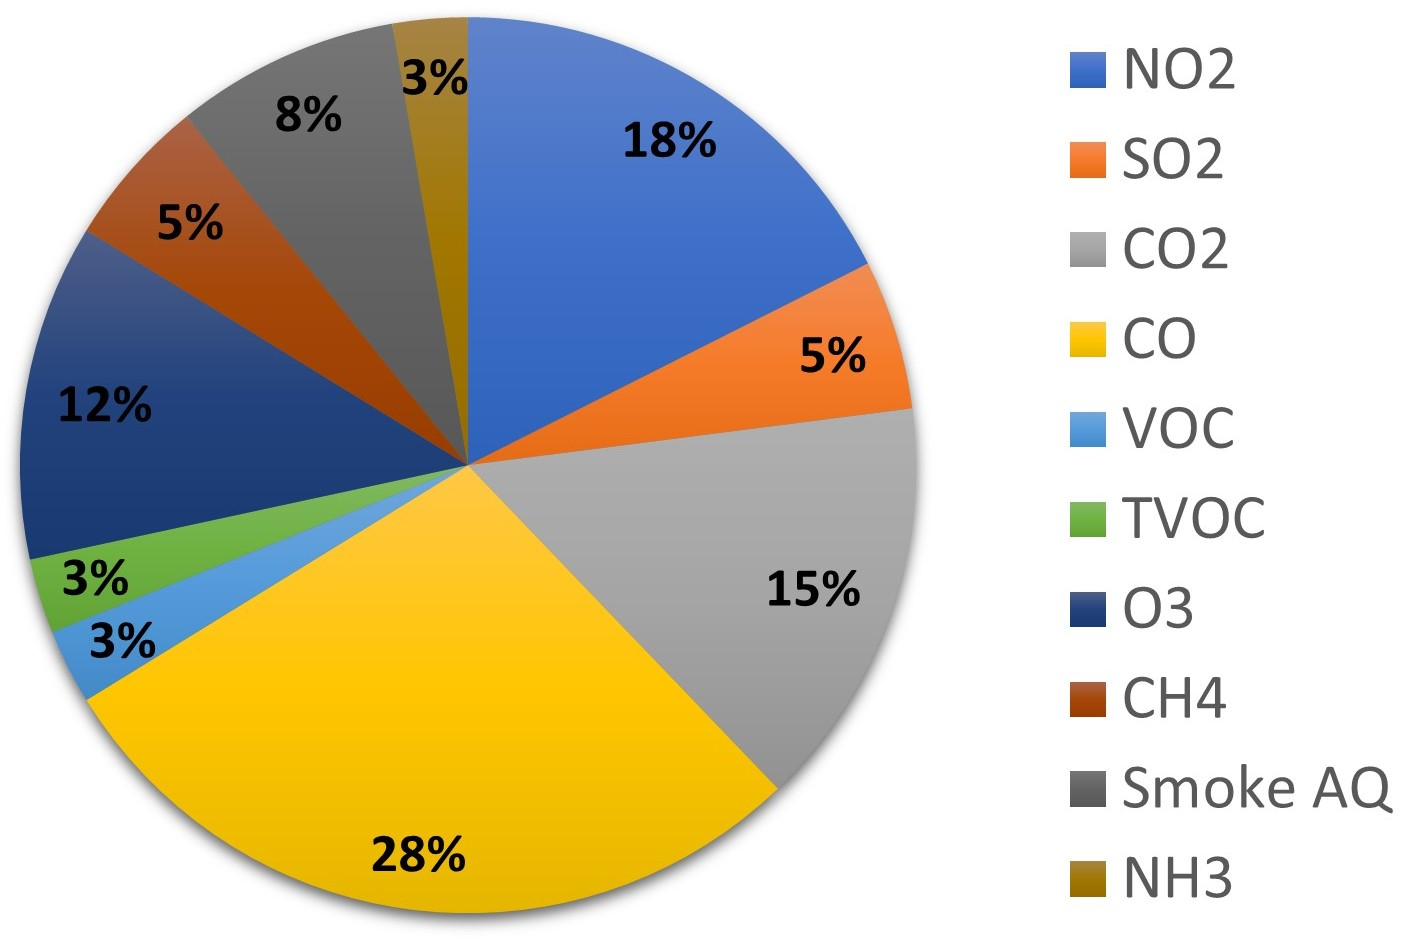
\includegraphics[width=0.7\linewidth]{percentage_occurences_pollutants.jpg}
%	\vspace*{6pt}
	\caption{Percentage of pollutants occurrences.}
        \label{occurrences_pollutants}
\end{figure}
\begin{table}[]
	\caption{European Union and the World Health Organization gas exposure limits.}
	\label{tabGAS}
	\centering
	\begin{tabularx}{\columnwidth}{lCCCC}
		\toprule
		& \multicolumn{4}{c}{Concentration (\unit{\ug\per\meter\tothe{3}})}\\
		& \multicolumn{2}{c}{EU~\cite{2008/50/EC}}	& \multicolumn{2}{c}{WHO~\cite{WHO}}\\
		Gas& One day	& Annual& One day& Annual\\
		\midrule
		CO        &  - & - & 0.004& - \\
		NO$_{2}$  & - &  40 & 25 &  10 \\
		SO$_{2}$  &  125 & - & 40 & - \\
		O$_{3}$   & 120 & - & 100  & -\\
		\bottomrule
	\end{tabularx}
\end{table}

In Table~\ref{tabGAS}, is presented the current standards set by the European Union and the World Health Organization for the gases that significantly impact breathable air and were included in the analyzed systems. The WHO guidelines where revised and updated in 2021, expecting to have a big impact and save people's lives. The ozone limits, imply a  concentration exposure to a 8 hour-mean.


\begin{table*}[tb]
	\caption{Comparison between carbon monoxide sensors.}
	\label{tabCOsensor}
	\centering
	\begin{tabular}{{p{3cm}p{1.5cm}p{1.5cm}p{1.5cm}p{1.5cm}p{2cm}p{1.5cm}p{2cm}}}
		\toprule
		Sensor name	& Ope. Range (\unit{ppm})& Response time (\unit{\s})& Ope. Temp. Range (\unit{\degreeCelsius})     & Ope. Hum. Range (\unit{\percent\ RH})& Sensor type& Approx. price (\$) & Brand name\\
		\midrule
		MQ2~\cite{MQ2} & 200-10000 & 90 & -20-50 & $<$95 & Semiconductor & 8 & Winsen       Elect.\\
		MQ7~\cite{MQ7} & 10-500 & 90 & -20-50 & $<$95 & Semiconductor & 8 & Winsen Elect.\\
		MQ9~\cite{MQ9} & 10-1000 & 90 & -20-50 & $<$95 & Semiconductor & 8 & Hanwei Elect.\\
		EC4-500-CO~\cite{EC4500CO} & 0-500 & $<$90 & -20-50 & 15-90 & Electrochemical & 95 & SGX \\
		CO-B4~\cite{COB4} & 1000 & $<$30 & -30-50 & 15-90 & Electrochemical & 75 & Alphasense\\
		MiCS-4514~\cite{MICS4514} & 1-1000 & 30 & -30-85 & 5-95 & MEMS & 13 & SGX \\
		MiCS-6814~\cite{MICS6814} & 1-1000 & 30 & -30-85 & 5-95 & MEMS & 13 & SGX \\
		DGS-CO 968-034~\cite{DGSCO968034} & 0-1000 & 15 & -20-40 & 15-95 & Electrochemical & 150 & SPEC Sensors\\
		\bottomrule
	\end{tabular}
\end{table*}




Since CO corresponded to the most analyzed gas in the selected projects, Table~\ref{tabCOsensor} collects and presents a comparison between the characteristics of all the used sensors among the different systems under study.

Nitrogen dioxide was the second most measured gas in the systems, the same analysis as before was conducted for this gas in Table~\ref{tabNO2sensor}. In fact, sensors MiCS-6814 and MiCS-4514, are both used for measuring CO and NO$_{2}$. It is interesting to notice that authors chose sensors basically from the same brands and as they are low-cost sensors, prices are under $\$$200. The information referred as NA, was not provided in the sensor's technical sheets.

\begin{table*}[!h]
	\caption{Comparison between nitrogen dioxide sensors.}
        \label{tabNO2sensor}
	\centering
    \begin{tabular}{p{3cm}p{1.5cm}p{1.5cm}p{1.5cm}p{1.5cm}p{2cm}p{1.5cm}p{2cm}}
        \toprule
	Sensor name	& Ope. Range (\unit{ppm})& Response time (\unit{\s})& Ope. Temp. Range (\unit{\degreeCelsius})     & Ope. Hum. Range (\unit{\percent\ RH})& Sensor type& Approx. price (\$) & Brand name\\
        \midrule
	MiCS-4514~\cite{MICS4514} & 0.05-10 & 30 & -30-85 & 5-95 & MEMS & 13 & SGX \\
	MiCS-2714~\cite{MICS2714} & 0.05-10 & 30 & -30-85 & 5-95 & MEMS & 11 & SGX \\
	MiCS-6814~\cite{MICS6814} & 0.05-10 & 30 & -30-85 & 5-95 & MEMS & 13 & SGX \\
	NO2-A43F~\cite{NO2A43F} & 0-20 & $<$80 & -30-40 & 15-85 & Electrochemical & 100 & Alphasense.\\
	NO2-B42F~\cite{NO2B42F} & 0-20 & $<$70 & -30-40 & 15-85 & Electrochemical & 100 & Alphasense\\
	ZMOD4410~\cite{ZMOD4410} & 0.02-0.5 (non selective) & NA & -20-50 & 5-90 & MEMS & 8 & Renesas Elect.\\
	EC4-20-NO2~\cite{EC4-20-NO2} & 0-20 & $<$35 & -20-50 & 15-90 & Electrochemical & 130 & SGX\\
	WSP-1110~\cite{WSP-1110} & 0.1-10 & NA & 20$\pm$2 & 65$\pm$5 & Semiconductor & 55 & Winsen Elect \\
	DGS-NO2 968-043~\cite{DGS-NO2-968-043} & 0-5 & $<$30 & -20-40 & 15-95 & Electrochemical & 80 & SPEC Sensors\\
	\bottomrule
    \end{tabular}
\end{table*}

As shown in Table~\ref{tabCOsensor} and Table~\ref{tabNO2sensor} gas sensors are basically of three types: semiconductor based, electrochemical, or MEMS.

For the semiconductor-based sensor technologies, the most used are the Metal-Oxide Semiconductor (MOS) technologies that base their operating principle on the change in the physico-chemical properties of the device when it comes into contact with the target gas. In the same, the variation of the conductivity of the semiconductor directly exposed to the gas is found, following reduction reactions that take place on the surface of the device. These sensors consist of a heating element, electrically separated from the sensing material (for example tin dioxide $\mathrm{SnO_2}$) through an insulating layer. Once the sensitive element composed of a thin layer of dioxide has been heated, the oxygen present in the air is attracted by the donor atoms and adsorbed, or accumulated on the outer layer of the sensitive element, thus, reducing the flow of charges inside the material. When the gas to be detected is present in the air, there is a variation in the conductivity of the semiconductor because the gas molecules bind to the oxygen molecules present on the surface of the sensor. This causes the electric charges previously bound to the semiconductor surface to be free to move and produce a current flow. The concentration of carriers that make up the current and therefore the consequent change in conductivity of the dioxide is directly proportional to the concentration of the target gas, as a result of which there is a decrease in the resistance value of the sensor. MOS technology sensors are very resistant, they are low-cost and easy to interface with a control system. Due to the high sensitivity of this type of sensor to the presence of humidity in the air, most of the applications mainly concern indoor~\cite{PM25_5} monitoring: the intervention of the water present in the air causes the concentration of gas perceived by the sensor to be compromised. Furthermore, due to greater interaction of the target gas molecules with those of H$_2$O present in humid environments, long exposure in such environments could "dirty" the chemical qualities of the device due to the bond established between the higher concentration of oxygen in humid environments with the donor atoms of the dioxide.

Electrochemical sensors consist of three electrodes: the working electrode WE, the counter electrode CE, the membrane placed between the two, and the auxiliary electrode mainly used to counterbalance the effects of temperature on the sensor. The operating principle of these sensors is based on the balancing of the currents produced by the two active electrodes (WE and CE) as a result of redox reactions which occur when the membrane in the medium comes into contact with the target gas. In clean air conditions, the currents created between the counter electrode and the working electrode are equal and opposite, unlike what happens when an oxide-reducing gas is present in the air. In this condition, one of the two currents will prevail over the other and its intensity will be directly proportional to the concentration of the gas to be detected. Electrochemical sensors are advantageous as they only require power for the potentiostatic circuit converting gas-induced current into an easily measurable voltage. The presence of the third electrode (AE) makes it possible to counterbalance the effects due to the variation in temperature and humidity of the environment in which these sensors work. Although both are subject to variations in climatic conditions, unlike MOS technology sensors, electrochemical ones do not incur the so-called "poisoning" or poisoning of the sensitive device due to the increase in pollutant molecules present in the air. This condition, which makes it necessary to replace the sensor, can only occur in the presence of target gas concentrations beyond the limits that can be tolerated by the sensor itself and indicated by the measurement range of the single gas. These characteristics make this technology more suitable than the previous one for monitoring applications, above all for external environments where temperature and humidity are highly variable and for which it is easy to counterbalance the effects by correcting the measurements. Another advantage of this technology is that it is much more selective than MOS technology to different types of gas and more sensitive as the presence of compounds to be monitored is detected even at lower concentrations.

Micro-ElectroMechanical Systems (MEMS) are extremely small devices in which all the internal components have micrometric dimensions (from the sensor portion to the circuitry necessary for signal conditioning and interfacing with the outside world) and for their operation they use mechanical structures capable of detecting and measuring physical and chemical quantities. In the presence of gas molecules in the air, there is a change in the morphology of the sensor surface which will be measured through various electrochemical or optical technologies, already mentioned, or acoustic, to obtain the gas concentration.
MEMS solutions are widely used for the construction of acceleration, pressure, optical, and even gas sensors. The advantage of these sensors is that they are very small, which makes them easy to integrate, very light, and cheap. The realization of the entire system on a single device also allows to lower the power consumption and the response times of the sensor. Due to the presence of metal lines and elements sensitive to humidity and thermomechanical stress, it is necessary to encapsulate these integrated circuits, due to this fragility, these sensors are excellent solutions for medical diagnosis, food testing, in the agricultural field, or monitoring of air quality in environments closed in which parameters such as humidity and temperature remain constant.

Within the sensing unit, particulate matter was also analyzed, revealing that at least one specific diameter of PM was measured in \qty{52}{\percent} of the analyzed works. Table~\ref{tabPMs} provides a summary of how often each type of particulate was measured and the number of different sensors used. It is striking that in all the systems where PM1, PM2.5, or PM10 were measured, different sensors were used only once, and just three sensors were used on more than one occasion.

\begin{table}[!b]
	\caption{Particulate matter occurrences.}
	\label{tabPMs}
	\centering
	\sffamily
    \begin{tabularx}{\columnwidth}{lCC}
        \toprule
	PM\therownum	& Occurrences & Number of different used sensors\\
	\midrule
	PM 1    & 3     &  2\\
	PM 2.5  & 10    & 9 \\
	PM 10   & 11    & 8  \\
	\bottomrule
    \end{tabularx}
\end{table}

Due to the importance of particulate matter for air quality analysis, Table~\ref{tabPMsensor} collects specific information from each sensor used in the reviewed systems. 
The operating principle of the sensors shown in Table~\ref{tabPMsensor} is Laser Light Scattering (LLS). This is a low-cost and low-power optical technology and allows PMs to be efficiently detected by scattering a laser beam when it encounters the particles in question. Sensors that exploit this principle are also called Optical Particle Counters (OPCs) and are very effective in counting particles of different sizes. Through a fan, air is introduced into the sensor, the particles thus transported pass through a laser beam causing the scattering of the light which will be detected and transformed by a photoelectric converter into an electrical impulse proportional to the size of the particle. The concentration of the latter instead will depend on the number of pulses with equal amplitude detected by the converter.

\begin{table}[]
	\caption{Low-cost particulate matter sensors.}
	\label{tabLCPMs}
	\centering
	\begin{tabularx}{\columnwidth}{lC}
		\toprule
		Manufacturer\therownum	& Sensors name\\
		\midrule	
		Alphasense      &   OPC-R1, OPC-R2, OPC-N3\\
		Omron electronic components &  B5W-LD0101-1/2      \\
		TeraSensor & Next-PM \\
		Sensirion & SEN5x \\
		Elitech & Temtop PM-900, Temtop PM-700, Temtop PM-300, Temtop PMJG-200 \\
		Panasonic & SN-GCJA5 \\
		Cubic Sensor and Instrument Co, Ltd.    &  PM2012SE-A/B, PM2016, PM2105L, PM2008-API, PM2008M-M, PM1003, PM1006K, PM1009, PM1010 \\
		Winsen &  ZH10-F Compact Laser Dust Sensor Module, ZH09 Laser dust sensor, ZH08 Laser dust sensor, ZH07 Laser dust sensor, \\
		\bottomrule
	\end{tabularx}
\end{table}

Although these sensors are generally low-cost and often insufficiently characterized in various scenarios, there are interesting approaches that make them appear as a rather compromising proposal. For example, in ~\cite{wang2015laboratory}, GP2Y1010AUOF, DSM501 and  PPD-\\42NS were tested under specific laboratory conditions and compared with reference equipment to validate results .This work showed that values between the reference equipment and the sensors were linearly correlated, obtaining an $R^2$ between 0.89 and 0.98, and also concluded that even accuracy and detection limits could be enhanced by improving the conditions of testing. 


\begin{table*}[!t]
	\caption{Comparison between particulate matter sensors.}
        \label{tabPMsensor}
	\centering
    \begin{tabular}{p{3cm}p{1.5cm}p{1.5cm}p{1.5cm}p{1.5cm}p{1.5cm}p{1.5cm}p{2.5cm}}
        \toprule
	Sensor name	& Detected particles (\unit{\um})& Resolution range (\unit{\ug\per\meter\tothe{3}}) &       Ope. Temp. Range (\unit{\degreeCelsius}) & Ope. Hum. Range (\%RH)& Operating principle&          Approx. price (\$) & Brand name\\
	\midrule
	PMS5003~\cite{PMS5003}\therownum & 1, 2.5, 10 & 1 & -10-60 & $<$90 & LLS     & 40 & Plantower\\
	PMS3003~\cite{PMS3003}\therownum& 1, 2.5, 10 & 1 & -10-60  & $<$90 & LLS  & 30 & Plantower \\
	PMSA003~\cite{PMSA0003} & 1, 2.5, 10 & 1 & -10-60 & $<$99 & LLS & 15 & Plantower \\
	%
	GP2Y1010AUOF~\cite{GP2Y1010AU0F} & 10 & Noise limit & -10-65 & NA & LLS & 20 & Sharp \\
	DSM501~\cite{DSM501} & 1,  2.5, 10& 1 & -10-65 & $<$95 & LLS & 12 & Samyoung S\&C\\
	%
	PPD42NS~\cite{PPD42NS} & 2.5 & 1  & 0-45 & $<$95 & LLS & 10 & Shinyei \\
	SDS 011~\cite{SDS011} &2.5, 10  &  0.3 & -20-50 & NA  & LLS & 27 & Nova Fitness Co\\
	%
	HPM32322550~\cite{HPM32322550} & 2.5, 10 & 1 & -10-50 & $<$95 & LLS & NA & Honeywell\\
	HPMA115S0-XX~\cite{HPM32322550} & 2.5, 10 & 1 & -20-50 & $<$95 & LLS & 58 & Honeywell\\
	\bottomrule
	\end{tabular}
\end{table*}

Table~\ref{tabLCPMs} shows a list of other manufacturers and the main low-cost sensors they fabricate for measuring different size diameters of particulate matter. This data allows us to realize the extensive range of sensors available in the market and it is noteworthy that new ones are continually being developed. 



Further requirements in the specifications of each sensor need to accomplish, as mentioned before, with the target of the project, directives, and standards of each country or the World Health Organization. Moreover, it is highlighted that a specific conversion equation is required in case the sensor gives as a result the particle count per unit volume.
 In Table~\ref{tabPM2.5} are presented the limits for PM2.5 in some countries and as a reference the WHO standards.

\begin{table}[!b]
	\caption{Current Standards for PM2.5.}
	\label{tabPM2.5}
	\centering
    \begin{tabularx}{\columnwidth}{lCC}
        \toprule
         Country - Region& One day (\unit{\ug\per\meter\tothe{3}})	& Annual (\unit{\ug\per\meter\tothe{3}})\\
        \midrule	
        European Union~\cite{2008/50/EC}   &  -  & 25 \\
        USA ~\cite{epa}			           &  35 & 12     \\
        China~\cite{china}                 & 75  & 35\\
        Japan~\cite{japan}                 & 35  &  15 \\
        Australia~\cite{australia}         & 25  & 8  \\
        Brasil~\cite{siciliano2020updated} & 25  &10 \\
        WHO~\cite{WHO}                     & 25  & 10 \\
	\bottomrule
    \end{tabularx}
\end{table}

Table~\ref{tabPM10} shows the same information as above but in this case the standards for PM10.

\begin{table}[!b]
	\caption{Current Standards for PM10}
	\label{tabPM10}
	\centering
		%\rowcolors{1}{gray!19}{white}
    \begin{tabularx}{\columnwidth}{lCC}
        \toprule
        Country - Region\therownum & One day (\unit{\ug\per\meter\tothe{3}})	& Annual (\unit{\ug\per\meter\tothe{3}})\\
        \midrule	
        European Union~\cite{2008/50/EC}   &  50   & 40 \\
        USA~\cite{epa}                     &  150  & -   \\
        China~\cite{china}                 &  150  &  70\\
        Japan~\cite{japan}                 &  100  & - \\
        Australia~\cite{australia}         &  50   & 25\\
        Brasil~\cite{siciliano2020updated} &  50   & 20\\
        WHO~\cite{WHO}                     &  50   & 20 \\
	\bottomrule
    \end{tabularx}
\end{table}

It is important to highlight that for both PM2.5 and PM10, although each country has established its own standards, the WHO standards serve not only as a reference but also set the most stringent values.

\subsection{Processing Unit Analysis}\label{PUA}

A similar analysis was conducted,  this time focusing on the processing unit within the sensor node. Specifically, the processing unit is implemented into a microcontroller that is the heart of the sensor node or the platform that will have to acquire, process, and transmit the data coming from the sensors. The choice of a device suitable for this purpose is based on a trade-off between cost and performance and, above all in the early design phases in which it is necessary to create a prototype of the overall system, choose low-cost, low-cost solutions power and open source for writing firmware fast and easy turns out to be quite beneficial. By considering this, the results, as presented in Table~\ref{tabPUA}, indicates that Arduino, including UNO and Mega variants, emerged as the most commonly utilized platform. Node MCU 1.0 ESP8266 and Raspberry Pi~\cite{leccese1, leccese2} are also featured in the list, being employed in various systems. Notably, it was observed that the authors predominantly favored low-cost and open-source microcontrollers or microprocessors. Furthermore, the analysis revealed that approximately 30\% of the devices were used only once, indicating a diverse range of platforms employed across the selected works.

\begin{table}[!b]
	\caption{Processing Unit Analysis.}
	\label{tabPUA}
	\centering
    \begin{tabularx}{\columnwidth}{lCC}
        \toprule
        Processing unit	& Percentage of occurrences \%\\
        \midrule	
        Arduino UNO              & 37\\
        Arduino Mega             & 11\\
        Node MCU 1.0 ESP8266     & 11\\
        Raspberry Pi 2 Model B   & 7\\
        Unique Implementation    & 30\\
        Not specified            & 4\\
	\bottomrule
    \end{tabularx}
\end{table}

As mentioned above, Arduino was notably the preferred microcontroller. Since 2005, the Arduino project, when it was first started as a tool for students, has developed different boards with various specifications. Some of the advantages of Arduino is that its Integrated Development Environment (IDE) is platform independent, which means it can operate on Unix, Linux, and Windows operating System~\cite{7724514}. Due that Arduino UNO and Mega head our list, Table~\ref{tabArduino} specifies some of their main characteristics.

\begin{table}[!b]
	\caption{Arduino technical specifications.}
	\label{tabArduino}
	\centering
    \begin{tabularx}{\columnwidth}{lCC}
        \toprule
        Specification& Arduino UNO~\cite{ArduinoUNO}	& Arduino Mega~\cite{ArduinoMega} \\
        \midrule	
        Microcontroller         & ATmega328P    &  ATmega2560\\
        Operating Voltage [V]   & 5             &  5 \\
        Input voltage [V]       & 7-12          & 7-12\\
        Digital IO Pins         & 14            & 54\\
        Analog Input Pins       & 6             & 16\\
        DC Current per IO Pins [mA]        & 20 & 20\\
        Flash Memory [KB]        & 32            & 256\\
        Clock Speed [MHz]       & 16            & 16\\
	\bottomrule
    \end{tabularx}
\end{table}

\subsection{Communication Unit Analysis}\label{CUA}

Table~\ref{tabCOM} presents the frequency of usage for different types of communication technologies, along with some notable characteristics considered in the works~\cite{7279943, abinayaa2014case, horyachyy2017comparison, de2017lorawan}. The analysis reveals that authors generally favored WiFi as the preferred communication technology over others. This preference could be attributed to factors such as cost-effectiveness and alignment with the specific application requirements of the project.

\begin{table}[!b]
	\caption{Communication technologies.}
	\label{tabCOM}
	\centering
    \begin{tabular}{lccc}
        \toprule
        Technology	& Occurrences	& Technology Range & Data rate\\
        \midrule	
        WiFi& 11        & Middle range      & 54 Mbps  \\
        LoRaWAN& 3      & Long range        & 29 bps - 50kbps  \\
        GSM& 3          & Long range        & 9.6 - 14.4 kbps  \\
        Zigbee& 2       & Short range       & 250 kbps \\
        Bluetooth& 2    & Short range       & 1 Mbps \\
        BLE& 1          & Short range       & 1 Mbps \\
        Not specified   & 5& Not applicable & Not applicable \\
	\bottomrule
    \end{tabular}
\end{table}
        
Particularly, the ESP8266 WiFi module was the most used device in the implementation of the systems. This module is low-cost, with an integrated TCP/IP protocol stack, which allows any microcontroller to connect to a  WiFi network. Unfortunately, in 33\% of the research, devices were not specified. Table~\ref{tabDEV} shows information about the number of occurrences and the communication technologies they are based on. Devices that were found to be implemented in a single occasion include: Digibee, GSM Arduino Shield, RN4871, HC-06, Modtronix Lora inAir4.

\begin{table}[!b]
	\caption{Communication devices.}
	\label{tabDEV}
	\centering
    \begin{tabularx}{\columnwidth}{lC}
        \toprule
        Device	& Technology\\
        \midrule	
        ESP8266             & WiFi\\
        GSM modem SIM 900A  & GSM\\
        Dragino Lora Shield & LoRaWAN \\
        Xbee S2             & Zigbee \\
        Unique Implementation & NA \\
        Not specified       & NA\\
	\bottomrule
    \end{tabularx}
\end{table}

\subsection{Power Supply Unit Analysis}\label{PSUA}
Even though the components of an IoT system are generally low-power consumable devices, it is essential to find an appropriate power supply to assure the correct performance of the sensor node, because once the energy starts to deplete, the sensors node functionality can be compromised. The selection of the power supply for each system was guided by considerations  such as power consumption, operational hours, and the type of system, as discussed in Figure~\ref{type_systems}. The results reveal that 48\% of the systems exclusively employed batteries, with varying capacities. This preference could be attributed to its affordability, battery diversity in terms of types and capacities, as well as widespread market availability. However, using batteries has certain drawbacks: they require replacement due to limited energy capacity, consequently elevating cost; additionally, their disposal poses environmental concerns~\cite{somov2015powering}. 

As most wireless systems rely on batteries, the market offers different alternatives such as alkaline, rechargeable alkaline, nickel-cadmium, nickel metal hydride, and lithium-polymer (li-po) batteries. Each type of battery has its advantages and disadvantages, e.g. nickel-cadmium batteries are rechargeable but as they are made of cadmium they are expensive and toxic to the environment~\cite{wenqi2014power}. Although alkaline batteries are the most common batteries used in wireless sensor nodes they have a very limited lifetime, due to their fixed energy rating; rechargeable alkaline batteries appeared as a low-cost version of the previous one, however, their energy density decreases rapidly through each cycle~\cite{wenqi2014power}.  

Additionally, 7\% of the systems opted for a combination of batteries and photovoltaic solar panels. Another 11\% drew power from the electricity grid, primarily applicable to fixed systems. Unfortunately, the power supply for the remaining 34\% of systems was not specified in the available information.

\section{Discussion and Conclusions}

The aim of this paper was to analyze different proposals of systems that had been implemented for monitoring outdoor air quality. Since this is a topic that matters and concerns governments, companies, and citizens itself, it is expected that more researchers continue investing in it. It is therefore desirable that this information can be used as a guideline in future implementations, starting with the choice of the sensors, processing, communication, and power supply unit. 

According to the type of system, the most implemented ones were fixed systems. 
Temperature and humidity, unlike pressure, were measured in most systems, where DHT11 and DHT22 sensors predominate. Moreover, carbon monoxide, nitrogen dioxide, carbon dioxide, and ozone~\cite{ozone} were the most representative gases in these researches. Despite the fact that particulate matter is one of the most dangerous pollutants for humans, it was only measured in half of the analyzed systems. 

Regarding the processing unit, it is noteworthy to emphasize a strong inclination towards employing low-cost and open-source microcontrollers or microprocessors. WiFi emerged as the favored communication technology among the authors, but it is also needed to clarify that the third part of the analyzed systems did not specify the type of communication technology used. For energizing the systems, batteries, photovoltaic solar panels, and energy from the network were used. Unfortunately, the authors did not specifically describe this unit, and also the third part of the work did not give information on this.

Even though it is essential to validate the information collected from the system to ensure accuracy, this paper exhibits that only 25\% of the authors made a validation work with a reference equipment or station. The primary objective of developing an air quality monitoring system should be to ensure that it guarantees good air conditions once implemented in real scenarios. Hence, future works should not only focus on the creation of a prototype but also on meeting the limits, laws and regulations, such as country-specific regulations or those of the World Health Organization. However, it is also essential to consider that this could be likely due to the expenses it takes to make this task, as it is necessary to have the availability of reference equipment which is expensive to maintain and also calibrate. Further requirements, can also involve having qualified personnel for the correct treatment of the data.

In summary, this research yielded different options and variety for each component of the sensor node architecture, which in the end will depend on the project budget, the specific goals that need to be achieved.


\section*{acknowledgment} 

The authors would like to acknowledge the contribution received from the project ARMONIA ``Attività di Ricerca e Monitoraggio Orientate da un’iNfrastruttura di tecnologie dell’Informa-zione e della comunicazione (ICT) per la tutela dell’Ambiente''.\\ (https://armonia.iia.cnr.it). The ARMONIA project was launched thanks to the funds POR FESR-FSE CALABRIA 2014–2020, ASSE I. 

The authors would also like to acknowledge the contribution received from the project
PNRR, TECH4YOU - ``Technologies for Climate Change Adaptation and Quality of Life Improvement'', CUP H23C22000370006, Project Code: ECS\_00000009.

\AIBreakAtRef{96}
\bibliographystyle{../imeko_acta}
\bibliography{main}

\end{document} 
